\documentclass{beamer}
\usepackage[utf8]{inputenc}
\usepackage[english]{babel}
\usepackage[T1]{fontenc}
\usepackage{slide_helper}
\usepackage[super]{nth}
\usepackage{array}
\usepackage{wasysym}
\usepackage{pgfplots}
\pgfplotsset{compat=1.5} 
\usepgfplotslibrary{statistics}

\DeclareSymbolFont{extraup}{U}{zavm}{m}{n}
\DeclareMathSymbol{\varheart}{\mathalpha}{extraup}{86}
\DeclareMathSymbol{\vardiamond}{\mathalpha}{extraup}{87}
\DeclareMathSymbol{\varclub}{\mathalpha}{extraup}{84} 
\DeclareMathSymbol{\varspade}{\mathalpha}{extraup}{85}

\newcommand{\suitheart}[1][]{{\color{red}\text{#1}\varheart}}
\newcommand{\suitspade}[1][]{{\color{black}\text{#1}\spadesuit}}
\newcommand{\suitdiamond}[1][]{{\color{red}\text{#1}\vardiamond}}
\newcommand{\suitclub}[1][]{{\color{black}\text{#1}\varclub}}

\newcommand{\prob}[1]{P\left(#1\right)}
\newcommand{\condprob}[2]{\prob{#1~\middle|~#2}}
\newcommand{\comb}[2]{{_{#1}C_{#2}}}
\newcommand{\perm}[2]{_{#1}P_{#2}}

\title[MA205 - Section 5.1]{Probability Distributions}

\begin{document}
\begin{frame}
\titlepage
\end{frame}

\begin{frame}
\begin{definition}
A \textbf{random variable} is a variable (typically represented by $x$) that has a single numerical value, determined by chance, for each outcome of a procedure.
\end{definition}\pause

\begin{example}
Consider tossing a coin: We could get a heads or a tail.

\vspace{1mm}
If we let $x$ be the number of tails we get in a single flip, then
\begin{equation*}
x=
\begin{cases}
0 & \text{Heads} \\
1 & \text{Tails}
\end{cases}
\end{equation*}
\end{example}\pause

\begin{definition}
A \textbf{probability distribution} is a description that gives the probability for each value of the random variable. It is often expressed in the format of a table, formula, or graph.
\end{definition}
\end{frame}

\begin{frame}
\begin{definition}
A \textbf{discrete random variable} has a collection of values that is finite or countable.
\end{definition}\pause

\begin{block}{Note}
If there are infinitely many values, the number of values are countable if it is possible to count them individually. Think counting the number of coin tosses.
\end{block}\pause

\begin{definition}
A \textbf{continuous random variable} has infinitely many values, and the collection of values is not countable.
\end{definition}\pause

\begin{block}{Note}
If there are infinitely many values, the number of values are not countable if some of them are on a continuous scale. Think body temperatures.
\end{block}\pause
\end{frame}

\begin{frame}
\begin{block}{Note}
We will be dealing almost exclusively with discrete random variables in this chapter.
\end{block}\pause

\begin{block}{Requirements}
Every probability distribution must satisfy the following requirements.
\begin{enumerate}
\item There is a numerical random variable $x$, and its number values are associated with corresponding probabilities.\pause
\item $\sum \prob{x}\approx 1$ where $x$ assumes all possible values.\pause
\item $0\leq\prob{x}\leq 1$ for every individual value of the random variable $x$.
\end{enumerate}
\end{block}
\end{frame}

\begin{frame}
\begin{example}
Let's consider tossing two coins, with the following random variable:
\begin{equation*}
x=\text{number of heads when two coins are tossed}
\end{equation*}\pause
With two coins tossed, the number of heads can be 0, 1, or 2, so $x$ is a discrete random variable. The table gives the probability distribution.
\begin{center}
\begin{tabular}{|c|c|}\hline
\textbf{Number of Heads} & $\boldsymbol{\prob{x}}$ \\\hline
0 & 0.25 \\
1 & 0.50 \\
2 & 0.25\\\hline
\end{tabular}
\end{center}\pause

We can check the requirements.
\begin{enumerate}
\item The variable $x$ is a numerical random variable, and its values are associated with probabilities.\pause
\item $\sum \prob{x}=0.25+0.50+0.25=1$\pause
\item Each value of $\prob{x}$ is between 0 and 1.
\end{enumerate}
\end{example}
\end{frame}

\begin{frame}
\begin{block}{Ways to display probability distributions.}
A \textbf{probability table}:

\vspace{-3mm}
\begin{center}
\begin{tabular}{|c|c|}\hline
\textbf{Number of Heads} & $\boldsymbol{\prob{x}}$ \\\hline
0 & 0.25 \\
1 & 0.50 \\
2 & 0.25\\\hline
\end{tabular}
\end{center}\pause

A \textbf{probability histogram}:
\begin{center}
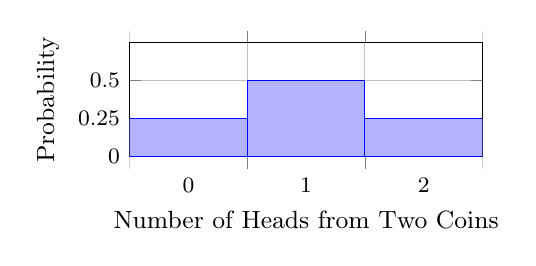
\begin{tikzpicture}
\begin{axis}[
small,
height=0.25\linewidth,
width=0.5\linewidth,
ybar interval,
ymajorgrids=true,
ylabel={Probability},
xlabel={Number of Heads from Two Coins},
ytick={0.00,0.25,0.50},
ymin=0,
ymax=0.75,
xmin=0,
xmax=3,
]
\addplot coordinates { (0, 0.25) (1, 0.50) (2, 0.25) (3,0) };
\end{axis}
\end{tikzpicture}
\end{center}\pause

A \textbf{probability formula}, where $x$ can be 0, 1, 2:

\vspace{-4mm}
\begin{equation*}
\prob{x}=\dfrac{1}{2(2-x)!x!}
\end{equation*}
\end{block}
\end{frame}

\begin{frame}
\begin{example}
Hiring managers were asked to identify the biggest mistakes that job applicants make during an interview. The table is based on their responses.
\begin{center}
\begin{tabular}{|l|c|}\hline
\multicolumn{1}{|c|}{$\boldsymbol{x}$} & $\boldsymbol{\prob{x}}$ \\\hline
\text{Inappropriate attire} & 0.50 \\
\text{Being late} & 0.44 \\
\text{Lack of Eye Contact} & 0.33 \\
\text{Checking phone or texting} & 0.30 \\
\textbf{Total} & \textbf{1.57}\\\hline
\end{tabular}
\end{center}
Does this table describe a probability distribution?\pause

\vspace{1mm}
We can check the requirements.
\begin{enumerate}
\item The variable $x$ is not numerical. The values are categorical.\pause
\item $\sum \prob{x}=1.57\neq 1$\pause
\item Each value of $\prob{x}$ is between 0 and 1.\pause
\end{enumerate}
Since not all three are satisfied, we see this table \emph{does not} describe a probability distribution.
\end{example}
\end{frame}

\begin{frame}
\begin{block}{Note}
A probability distribution describes a population instead of a sample.
\end{block}\pause

\begin{block}{Mean $\mu$ for a Probability Distribution}
\begin{equation*}
\mu = \sum\left(x\cdot\prob{x}\right)
\end{equation*}
\end{block}\pause

\begin{block}{Variance $\sigma^2$ for a Probability Distribution}
\begin{equation*}
\sigma^2=\sum\left({(x-\mu)}^2\cdot\prob{x}\right)=\sum\left(x^2\cdot\prob{x}\right)-\mu^2
\end{equation*}
\end{block}\pause

\begin{block}{Standard Deviation $\sigma$ for a Probability Distribution}
\begin{equation*}
\sigma=\sqrt{\sum\left(x^2\cdot\prob{x}\right)-\mu^2}
\end{equation*}
\end{block}\pause

\begin{block}{Round-Off Rule}
Round results by carrying \emph{one or more decimal place} than the number of decimal places used for the random variable $x$.
\end{block}
\end{frame}

\begin{frame}
\begin{example}
In the casino game Roulette, a wheel with 38 spaces (18 red, 18 black, and 2 green) is spun. In one possible bet, the players bet \$1 on a single number. If that number is spun on the wheel, then they receive \$36. Otherwise, they lose their \$1.

\vspace{2mm}
On average, how much money should a player expect to win or lose if they play this game repeatedly?\pause

\vspace{2mm}
Any number you bet on will have the following probabilities:
\begin{center}
\begin{tabular}{|c|c|} \hline
Outcome & Probability \\ \hline
\$35 (win) & 1/38 \\\hline
-\$1 (lose) & 37/38 \\ \hline
\end{tabular}
\end{center}\pause

So, \textbf{on average}, we will have a net change of
\begin{equation*}
\$35\cdot\dfrac{1}{38} + -\$1\cdot\dfrac{37}{38} = \$0.9211 - \$0.9737 \approx -\$0.053
\end{equation*}

That is, \textbf{on average}, we will lose 5.3 cents per space we bet on.
\end{example}
\end{frame}

\begin{frame}
\begin{definition}
The \textbf{expected value} of a discrete random variable $x$ is denoted by $E$, and it is the mean value of the outcomes, so $E=\mu$.
\begin{equation*}
E=\sum\left(x\cdot\prob{x}\right)
\end{equation*}
\end{definition}\pause

\begin{block}{Caution}
An expected value need not be a whole number, even if the different possible values of $x$ might all be whole numbers.
\end{block}
\end{frame}

\begin{frame}
\begin{example}
Consider a lottery where balls numbered 1 through 48 are placed in a machine and six balls are drawn at random. If the six numbers drawn match the numbers that a player has chosen, that player wins \$1,000,000. If they match five numbers, they win \$1,000. A lottery ticket costs \$1.\\ Let us calculate the expected value.\pause

\vspace{2mm}
The following table gives the values and probabilities.
\begin{center}
{%
\setlength{\extrarowheight}{1.3mm}
\begin{tabular}{|l|c|r|} \hline
Outcome & Value & Probability\\ \hline
Match all six & \phantom{-}\$999,999 & $\tfrac{\comb{6}{6}}{\comb{48}{6}}=\tfrac{1}{12272512}$ \\[1.3mm] \hline
Match five & \phantom{-}\$999\phantom{999,} & $\tfrac{\left(\comb{6}{5}\right)\left(\comb{42}{1}\right)}{\comb{48}{6}}=\tfrac{252}{12272512}$ \\[1.3mm] \hline
Match four for fewer & -\$1\phantom{99,999} & $1-\tfrac{253}{12272512} = \tfrac{12271259}{12272512}$ \\[1.3mm] \hline
\end{tabular}
}
\end{center}\pause
The expected value is then:

\vspace{-7mm}
\begin{equation*}
\left(\$999,999\right)\cdot\tfrac{1}{12272512} + \left(\$999\right)\cdot\tfrac{252}{12272512} + \left(-\$1\right)\cdot\tfrac{12271259}{12272512} \approx -\$0.898
\end{equation*}

\vspace{-3mm}
So, on average, a player can expect to lose about 90 cents on a ticket.
\end{example}
\end{frame}

\begin{frame}
\begin{note}
It is generally a bad idea to play a game with a negative expected value.

\vspace{2mm}
A game is called \textbf{fair} if it's expected value is zero.
\end{note}\pause

\begin{example}
A friend offers to play a game, in which you roll 3 standard 6-sided dice. If all the dice roll different values, you give him \$1. If any two dice match values, you get \$2. Should you play this game?\pause

\vspace{2mm}
Suppose you roll the first die. The probabilities are:
\begin{equation*}
\begin{aligned}
\prob{\text{no match}} &= \dfrac{\left(\comb{6}{1}\right)\left(\comb{5}{1}\right)\left(\comb{4}{1}\right)}{\left(\comb{6}{1}\right)\left(\comb{6}{1}\right)\left(\comb{6}{1}\right)} = \dfrac{6\cdot5\cdot4}{6\cdot6\cdot6} = \dfrac{5}{9} &\left(\approx 55.5\%\right) \\
\prob{\text{at least two match}} &= 1 - \prob{\text{no match}} = 1-\dfrac{5}{9} = \dfrac{4}{9} &\left(\approx 44.4\%\right)
\end{aligned}
\end{equation*}\pause

\vspace{-5mm}
The expected value is:

\vspace{-5mm}
\begin{equation*}
\$2\cdot\dfrac{4}{9} -\$1\cdot\dfrac{5}{9} = \dfrac{1}{3} \approx \$0.33
\end{equation*}

\vspace{-1mm}
You will, on average, win 33 cents per play.
\end{example}
\end{frame}

\begin{frame}
\begin{example}
Suppose an individual has a 0.242\% risk of dying during the next year. An insurance company charges \$275 for a life-insurance policy that pays \$100,000 death benefit. What is the expected value for the person buying the insurance?\pause

\vspace{2mm}
The probabilities and values for the two outcomes are:
\begin{center}
\begin{tabular}{|r|r|} \hline
Value & Probability \\ \hline
\$100,000-\$275 = \$99,725 & 0.00242 \\ \hline
-\$275 & 1-0.00242 = 0.99758 \\ \hline
\end{tabular}
\end{center}\pause
The expected value is $\$99,725\cdot 0.00242 -\$275\cdot0.99758 = -\$33$.
\end{example}\pause
\begin{note}
It makes sense that a insurance policy would have a negative expected value, otherwise the insurance company couldn't stay in business.

\vspace{2mm}
The benefit for the consumer is the security that the policy provides.
\end{note}
\end{frame}

\begin{frame}
\begin{example}
A company estimates that 0.7\% of their products will fail after the original warranty period but within 2 years of the purchase, with a replacement cost of \$350. If they offer a 2 year extended warranty for \$48, what is the company's expected value?\pause

\vspace{2mm}
The probabilities and values for the two outcomes are:
\begin{center}
\begin{tabular}{|r|r|} \hline
Value & Probability \\ \hline
-\$350 + \$48 = -\$302 & 0.007 \\ \hline
\$48 & 1-0.007 = 0.993 \\ \hline
\end{tabular}
\end{center}\pause
The expected value is $-\$302\cdot 0.007 + \$48\cdot0.993 = \$45.55$.

\vspace{2mm}
The company makes, on average, \$45.55 on each extended warranty.
\end{example}\pause

\begin{note}
The expected value for the consumer may be different. The consumer is likely to pay the more to repair or replace the item out of warranty.\\ (The company pays manufacturing cost, consumer has to pay retail cost.)
\end{note}
\end{frame}

\begin{frame}
\begin{block}{Identifying Significant Results with Probabilities}
\begin{itemize}
\item $x$ successes among $n$ trials is a \emph{significantly high} number of successes if the probability of $x$ or more successes is 0.05 or less.
\item $x$ successes among $n$ trials is a \emph{significantly low} number of successes if the probability of $x$ or fewer successes is 0.05 or less.
\end{itemize}
\end{block}\pause

\begin{block}{The Rare Event Rule for Inferential Statistics}
If under a given assumption, the probability of a particular outcome is very small and the outcome occurs \emph{significantly less than} or \emph{significantly more than} what we expect with that assumption, we conclude that the assumption is probably not correct.
\end{block}
\end{frame}

\begin{frame}
\begin{example}
Is 252 heads in 460 coin tosses a significantly high number of heads?\pause

\vspace{1mm}
A result of 252 heads in 460 coin tosses is greater than we expect with random chance, but we need to determine whether 252 heads is significantly high.\pause

\vspace{1mm}
Here, the relevant probability is the probability of getting 252 or more heads in 460 coin tosses.
\vspace{-4mm}
\begin{equation*}
\prob{\text{255 or more heads in 460 coins}}=\dfrac{1}{2^{460}}\sum_{i=252}^{460} \comb{460}{i} = 0.0224
\end{equation*}\pause

\vspace{-5mm}
Since $0.0224 < 0.05$, 252 heads is significantly high.
\begin{center}
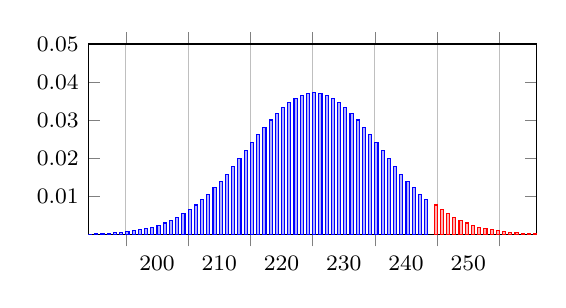
\begin{tikzpicture}
\begin{axis}[
small,
height=0.33\linewidth,
width=0.6\linewidth,
ybar interval,
%ymajorgrids=true,
ylabel={},
xlabel={},
ytick={0.01,0.02,0.03,0.04,0.05},
xtick={},
ymin=0,
ymax=0.05,
xmin=194,
xmax=266,
scaled ticks=false, tick label style={/pgf/number format/fixed}
]
\addplot coordinates { (194,0.00013135813782411948) (195,0.0001791859726216522) (196,0.00024226674869758804) (197,0.0003246620388638186) (198,0.0004312430112180934) (199,0.0005677671805986825) (200,0.0007409361706810694) (201,0.0009584248973986152) (202,0.001228871526862854) (203,0.0015618170144363949) (204,0.0019675831995590912) (205,0.002457079507742374) (206,0.0030415304586140766) (207,0.003732119499941053) (208,0.004539549199449088) (209,0.00547352343665463) (210,0.006542163726668157) (211,0.007751378823066251) (212,0.009104213806334248) (213,0.010600211380150206) (214,0.012234823415406607) (215,0.01399891423343937) (216,0.015878398088849555) (217,0.01785405130728485) (218,0.019901534255365554) (219,0.02199164972510775) (220,0.02409085265341863) (221,0.026162011931319513) (222,0.028165409241364445) (223,0.030059943495272298) (224,0.0318044937873984) (225,0.03335938015033914) (226,0.03468785104128928) (227,0.03575752045665738) (228,0.03654167660702647) (229,0.03702038852763392) (230,0.037181346738636455) (231,0.03702038852763392) (232,0.03654167660702647) (233,0.03575752045665738) (234,0.03468785104128928) (235,0.03335938015033914) (236,0.0318044937873984) (237,0.030059943495272298) (238,0.028165409241364445) (239,0.026162011931319513) (240,0.02409085265341863) (241,0.02199164972510775) (242,0.019901534255365554) (243,0.01785405130728485) (244,0.015878398088849555) (245,0.01399891423343937) (246,0.012234823415406607) (247,0.010600211380150206) (248,0.009104213806334248) (249,0)};
\addplot coordinates { (249,0.007751378823066251) (250,0.006542163726668157) (251,0.00547352343665463) (252,0.004539549199449088) (253,0.003732119499941053) (254,0.0030415304586140766) (255,0.002457079507742374) (256,0.0019675831995590912) (257,0.0015618170144363949) (258,0.001228871526862854) (259,0.0009584248973986152) (260,0.0007409361706810694) (261,0.0005677671805986825) (262,0.0004312430112180934) (263,0.0003246620388638186) (264,0.00024226674869758804) (265,0.0001791859726216522) (266,0.00013135813782411948)  };
\end{axis}
\end{tikzpicture}
\end{center}
\end{example}
\end{frame}
\end{document}
